\documentclass[9pt,twoside,lineno]{pnas-new}
% Use the lineno option to display guide line numbers if required.

\templatetype{pnassupportinginfo}

\title{Water resource utilization regimes at a basin scale: transition framework and development traps}
\author{Shuang Song, Shuai Wang, Bojie Fu, Xutong Wu (complete author list)}
\correspondingauthor{Shuai Wang.\\E-mail: shuaiwang@bnu.edu.cn}

\begin{document}

%% Comment out or remove this line before generating final copy for submission; this will also remove the warning re: "Consecutive odd pages found".
% \instructionspage

\maketitle

%% Adds the main heading for the SI text. Comment out this line if you do not have any supporting information text.
\SItext{This supplementary document consists of three sections and 10 figures. Firstly, we introduced our study area, the Yellow River Basin, in the section Methods S1. Definition of study area. Then, we give a detailed description of used datasets and analysis their uncertainties in the section Methods S2. Detailed information on dataset and processing. Finally, the index along with corresponding indicators are introduced in the section Methods S3. Water Utility Regime Index.}


% \subsection*{Brief description of Supplementary Information contents: }
% Type or paste text here. This should be additional explanatory text such as an extended technical description of results, full details of mathematical models, etc.   

% tag 研究区定义
\section*{Methods S1. Definition of study area}

\subsection*{Region divisions of Yellow River Basin}

The study area is the Yellow River Basin (YRB, see Fig. S1-A), which has experienced the most intense water exploitation and the most dramatic shifts of management regime in China. According to the Yellow River Conservancy Commission (YRCC), an administrative government directly under the Ministry of Water Resources at the basin level, the upper, middle and lower reaches of the Yellow River can be distinguished by characteristic of river. However, there is another scheme suggesting that the upstream only refers to river source areas with little human disturbance and high water retention capacity. Anyhow, since the socio-economic and natural conditions were considered in this study, we integrated the two schemes above and divided the Yellow River Basin into four regions, which can be distinguished by three important hydrological control stations (see Fig. S1-B). Previous studies have also shown that such a division is valid when both social water use and the natural conditions of the basin are considered, as the regions exhibit strong heterogeneity among themselves (see Fig. S1-C):

\begin{itemize}
    \item \textbf{Source Region (SR):} Over 50\% of natural runoff was produced in this region. The most ecology function here is water conservation, as sparsely populated and less economically developed.
    \item \textbf{Upper Region (UR):} With the highest per capita irrigated land area, there are numbers of large irrigation lands in this region. However, because of backward production methods, efficiency of irrigation are used to be very low.
    \item \textbf{Middle Region (MR):} Crossing Loess Plateau, famous rich-sand area, Yellow River loads most of its sediments here with the highest soil erosion risk. To reverse this situation, the grain for green project changed the water utilization here strikingly.
    \item \textbf{Lower Region (LR):} With dense population and the traditional agricultural trajectory, lower region used to be the largest water use region. However, as the industrial transformation going, proportion of agriculture keeps decreasing, but LR is still the largest water use region in each aspect.
\end{itemize}

In general, there are inter-regional differences in the economic layout, distribution of water resources, distribution of water consumption, and population distribution of the Yellow River Basin (see Fig. S2). On the basis of these fundamental differences, social development and watershed management continue to influence and reshape their changes, making the Yellow River Basin the world's most intimately connected and dramatically changing large river basin. Thus, as a case study for analysing the evolution of the human-water relationship, it possesses typicality.

\subsection*{Importance of water resource to society within the YRB}
Water resources make an irreplaceable contribution to the development of society in the YRB. Firstly, each aspect of economic development highly depended on water resources, since the most water use patterns are positively correlated with the region's key economic indicators (see Fig. S3-A). Secondly, their relationships have noticeably changed over the study period. In particular, the major water-consuming sectors have undergone particularly dramatic changes (see Fig. S3-B). 

% 举农业案例作为说明
%For an example, the agriculture, which occupied over 60\% of water consumptions, whose relationship with regional economic development has weakened, and there have been significant changes in water consumption per unit and total water consumption (see Fig. S).

\subsection*{Changes brought from human activities on the YRB}
Humans are constantly modifying the water cycle processes in the watersheds as society develops.
\begin{itemize}
    \item Firstly, the YRB has been subject to strong intervention by human activities since ancient times, while the last 60 years have seen the most dramatic changes. Under human influence, the Yellow River's surface runoff, sediment transport, and human water consumption patterns have all undergone multiple regime shifts in the last 60 years (see Fig. S4). 
    \item Secondly, landscapes in the YRB have significantly altered by human activities, which can both change the natural and the social water cycle (see Fig. S5). For an example, “grain for green” project has produced a significant change of landscapes in the middle region (MR) of YRB. With the addition of xxx hectares of forest in an erosion-prone area, water use patterns in the area and surface runoff patterns in the middle and lower reaches have been radically altered.
    \item Thirdly, a series of management practices have promoted in order to govern the YRB (see Fig. S6). Since the establishment of the Yellow River Water Conservancy Commission in XX, the agency has continued to reform and expand, eventually forming a basin management agency with unified coordination, scheduling and regulatory functions. Since the promulgation of the Water Law in xxx, the Ministry of Water Resources, the YRCC and other relevant agencies have issued a series of policies to carry out comprehensive river basin management under the guidance of national laws.
\end{itemize}
Historic and recent river basin management practices have strong impacts on water utilization.


% tag 数据集介绍
\section*{Methods S2. Detailed information on datasets}

Multiple types of dataset were used in this study (see Table S1). 
\subsection*{Statistical datasets}
% 使用了GDP数据,年鉴数据,还有从第二次水资源调查提取的数据
For statistics, we used GDP data, water resources uses data extracted from the 2nd National Water Resources Assessment Program \cite{zhouDecelerationChinaHuman2020} and statistical yearbook data of YRB.
GDP data from the China Macro data in the Wind database, which firstly aggregated from annual reports of the provinces. 
Water resources uses dataset was published by Zhou et al. \cite{zhouDecelerationChinaHuman2020}, which records water utilization in different sectors along with social-economic situations in perfects level. 
This dataset was mainly extracted by 2nd National Water Resources Assessment Program launched in 2002, led by the National Development and Reform Commission and the Ministry of Water Resources (see ref (1) and \url{http://www.mwr.gov.cn/english/publs/} for more details). Since then, the statistics from the survey using the same criteria have been supplemented and harmonized to the 2013 administrative divisions. 
%TODO xx 
The data covers a total of subcategories of water use under four broad categories: agriculture, industry, urban and rural, but does not distinguish between surface water and groundwater. There is uncertainty at the county scale for each disaggregated water use sector, but because the data are corrected for statistical information using the water balance method, the data are adequate for the regional scale and the four broad water use categories used in this study.
Finally, in order to make a simple distinction between the proportion of surface water and groundwater extraction where needed, we use basin-scale water resources annual reporting data. Yearbook data of YRB documenting surface water resources and groundwater resource extraction in each watershed and province. 


\subsection*{Hydrological datasets}
For hydrological datasets, reservoirs data and a measured runoff data were used in this study.
The reservoir dataset were collected by Wang et al. \cite{wangYellowRiverWater2019}, which introduced includes the major new reservoirs built in the Yellow River Basin since 1949. Of these, we consider the reservoirs marked as pivot projects by the YRCC to be more important, as they are directly involved in water resources management in the basin (\url{http://www.yrcc.gov.cn/hhyl/sngc/}). Annual runoff data derived from hydrological station measurements.

\subsection*{Political datasets}



% tag 数据处理
\section*{Methods S3. Harmonization of datasets}

% 指数介绍
\section*{Methods S4. Water Utility Regime Index}


\subsection*{Stress: SFV-index}
	% 提出了很多的指标度量水压力,如水资源压力指数,水资源xxx等
	Various metrics, therefore, proposed for water stress (e.g. water scarcity, water stresses index, scarcity-flexibility-variability index), where the dimensions of human impact are increasingly valued.
	% 其中SFV指数比较有用
    Among of them, by taking changes of water flexibility and variability into account,	the scarcity-flexibility-variability (SFV) index focus more on dynamic responses to water resources in developing perspective, which considered a valid indicator of temporal changes in water stresses.
    
\subsection*{Tendentiousness: Non-provisioning share}
	% xxx等人通过考虑消费品中的水消耗提出了虚拟水理论
	% 但随着水资源利用方式的变迁,在其基础上兴起的水足迹研究,则进一步泛化了水相关的产品和服务概念。
	% 如今,世界非产品形式供给于人类的水资源已达xx%,范围包含了xxxxxx等方式,人类在“消耗水”向“利用水”和的倾斜。

\section{Methods S4. Water Management Practices}

% tag 附录图

%%% Each figure should be on its own page
% 补充图片1:研究区示意图
\begin{figure}
    \centering
    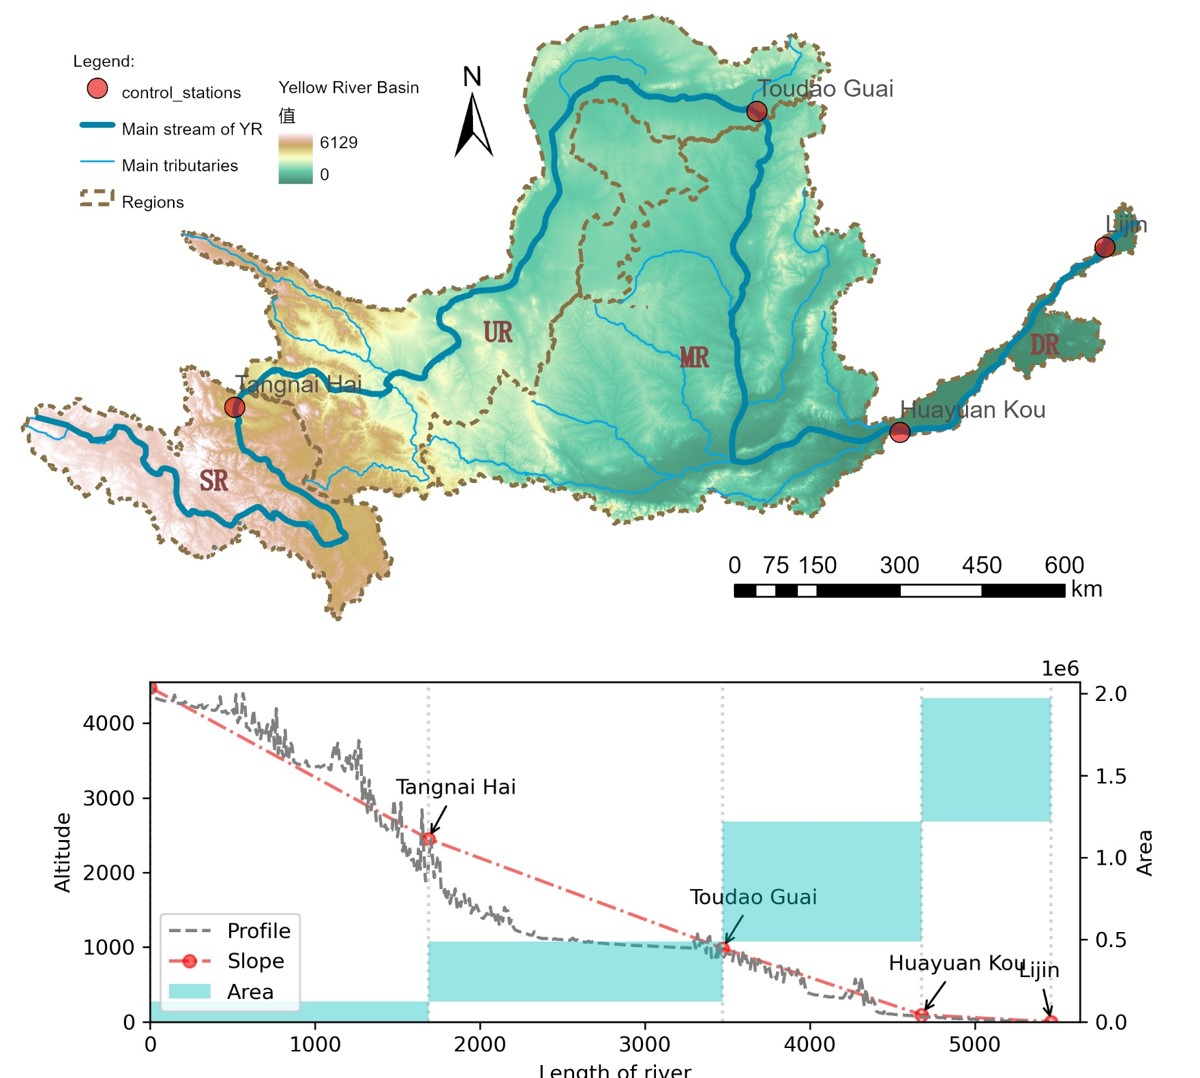
\includegraphics[width=\textwidth]{../../figures/supplementary_information/s1_study_area.jpg}
    \caption{Yellow River Basin}
\end{figure}

% 补充图片2:研究区分区特征
\begin{figure}
    \centering
    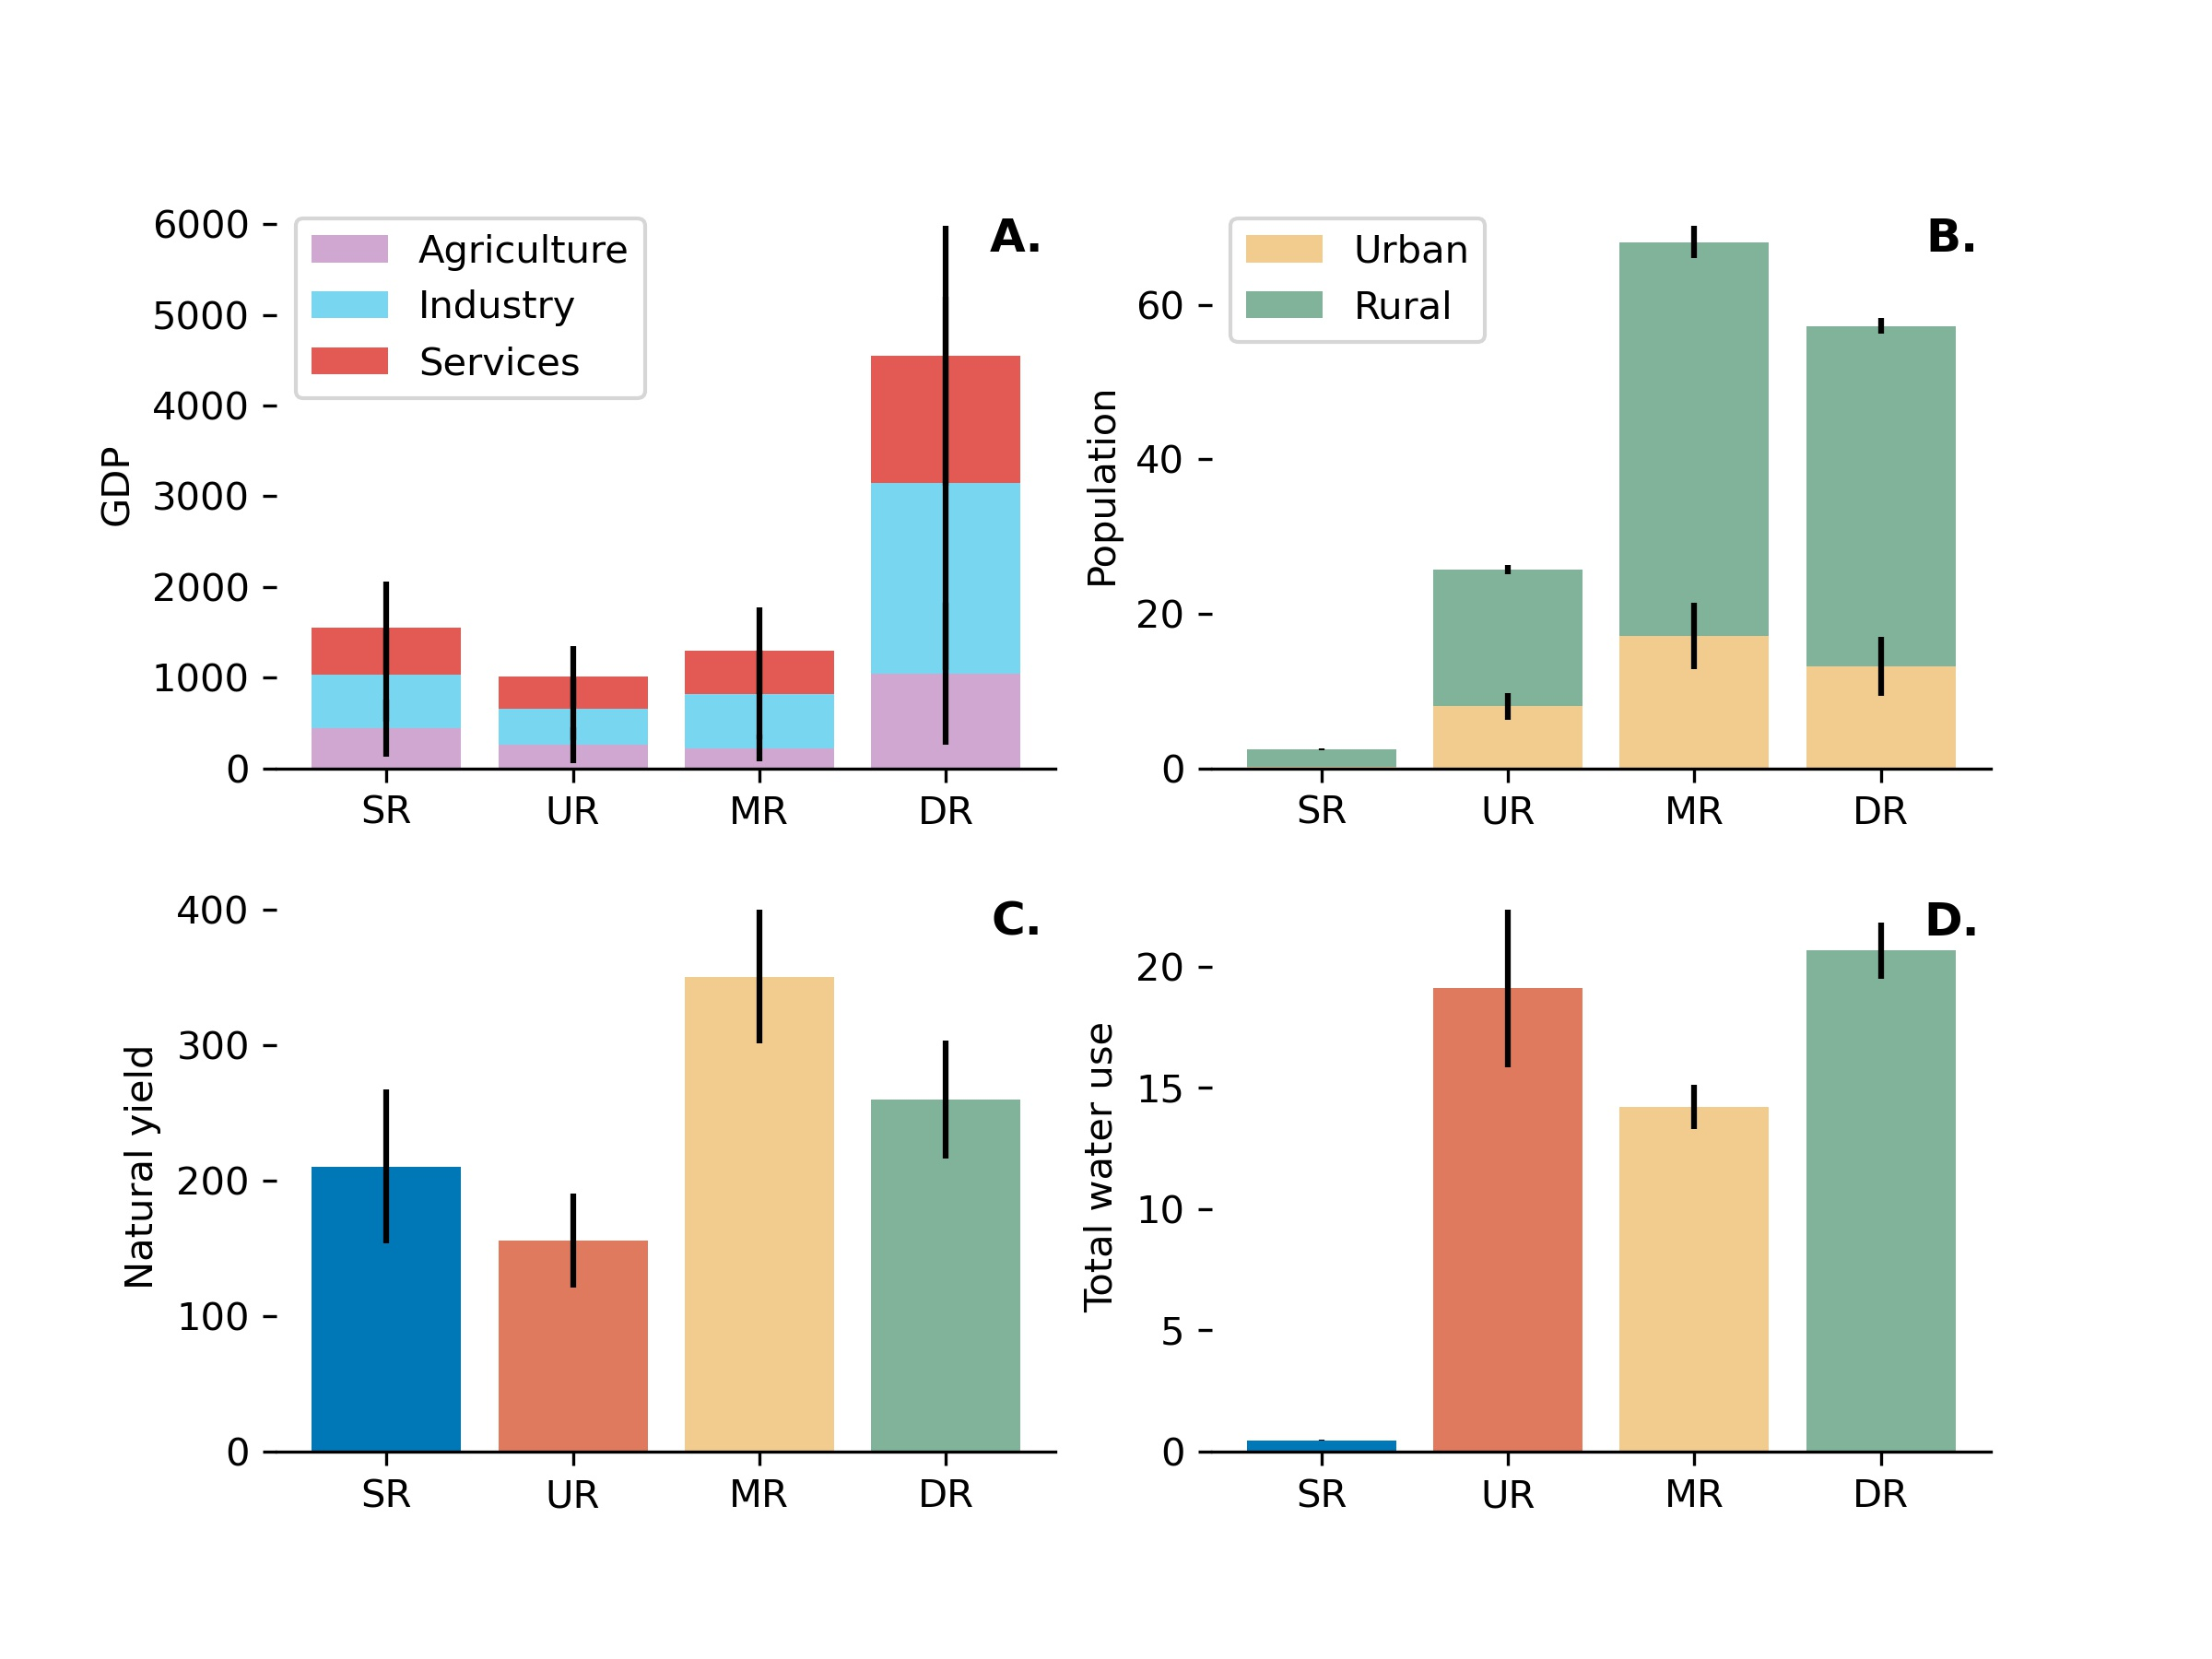
\includegraphics[width=\textwidth]{../../figures/supplementary_information/region_differences.jpg}
    \caption{Different regions}
\end{figure}


% 补充图片3:天然水资源量
\begin{figure}
    \centering
    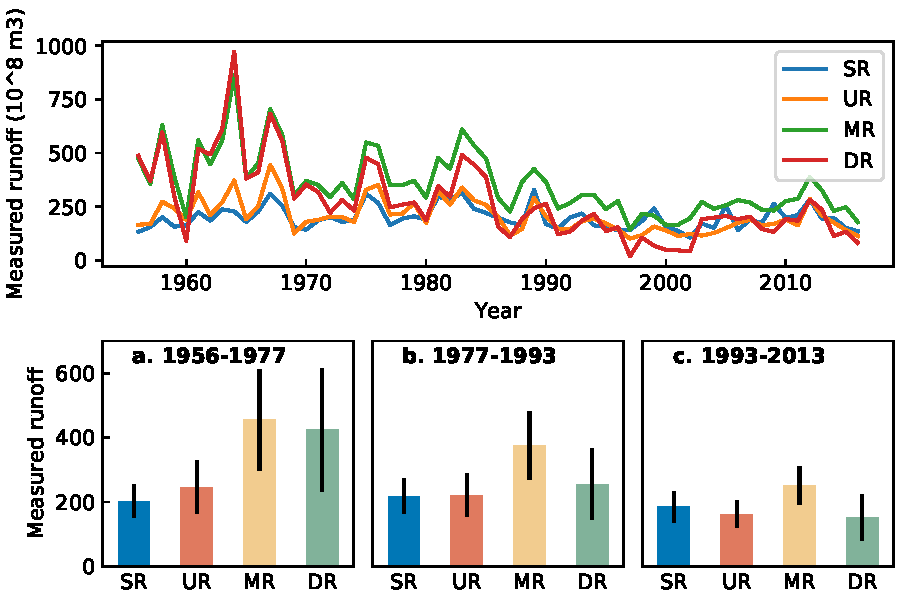
\includegraphics[width=\textwidth]{../../figures/supplementary_information/sf_measured_runoff.pdf}
    \caption{Natural measured runoff of Yellow River within different periods.}
\end{figure}


% 补充图片4:水资源灵活性
\begin{figure}
    \centering
    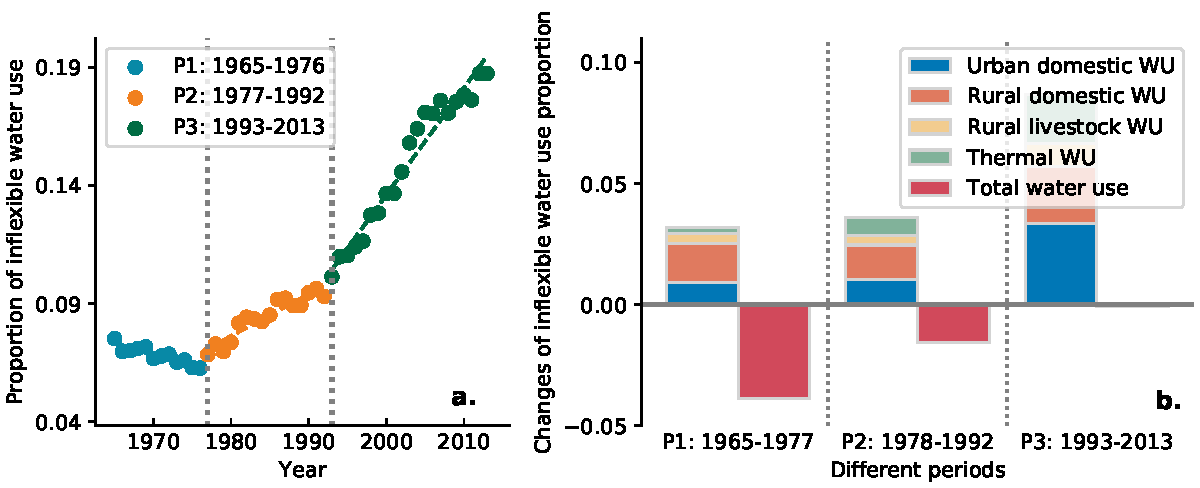
\includegraphics[width=0.95\textwidth]{../../figures/supplementary_information/inflexible_wu.pdf}
    \caption{Flexibility}
\end{figure}
    

% 补充图片5:水库数量和累积库容
\begin{figure}
    \centering
    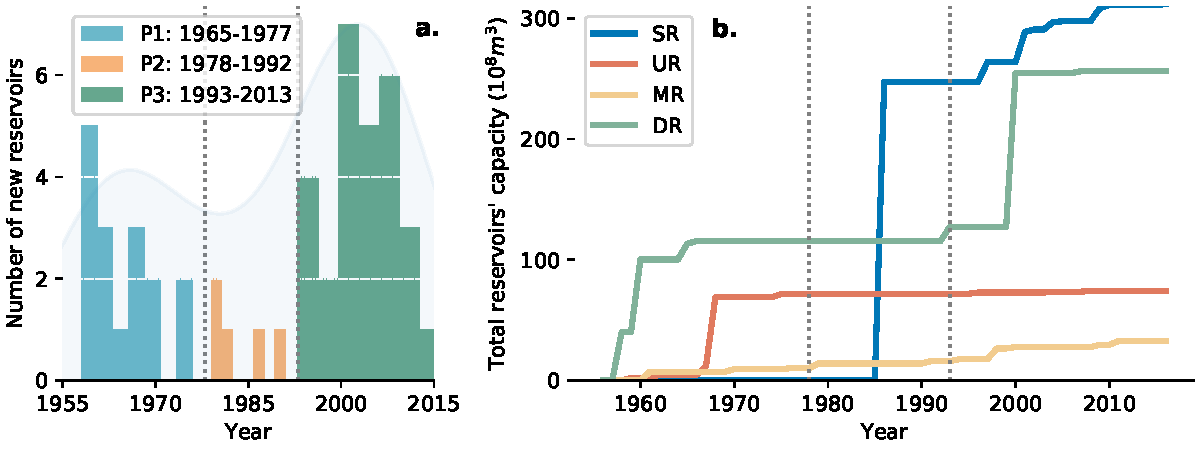
\includegraphics[width=0.95\textwidth]{../../figures/supplementary_information/reservoirs.pdf}
    \caption{Reservoirs and accumulated storage}
\end{figure}


% 补充图片6:节水措施
\begin{figure}
    \centering
    
\includegraphics[width=0.95\textwidth]{../../figures/placeholder_l.jpg}
    \caption{technological solutions and water conservation practices}
\end{figure}

% 补充图片7:用水比例
\begin{figure}
    \centering
    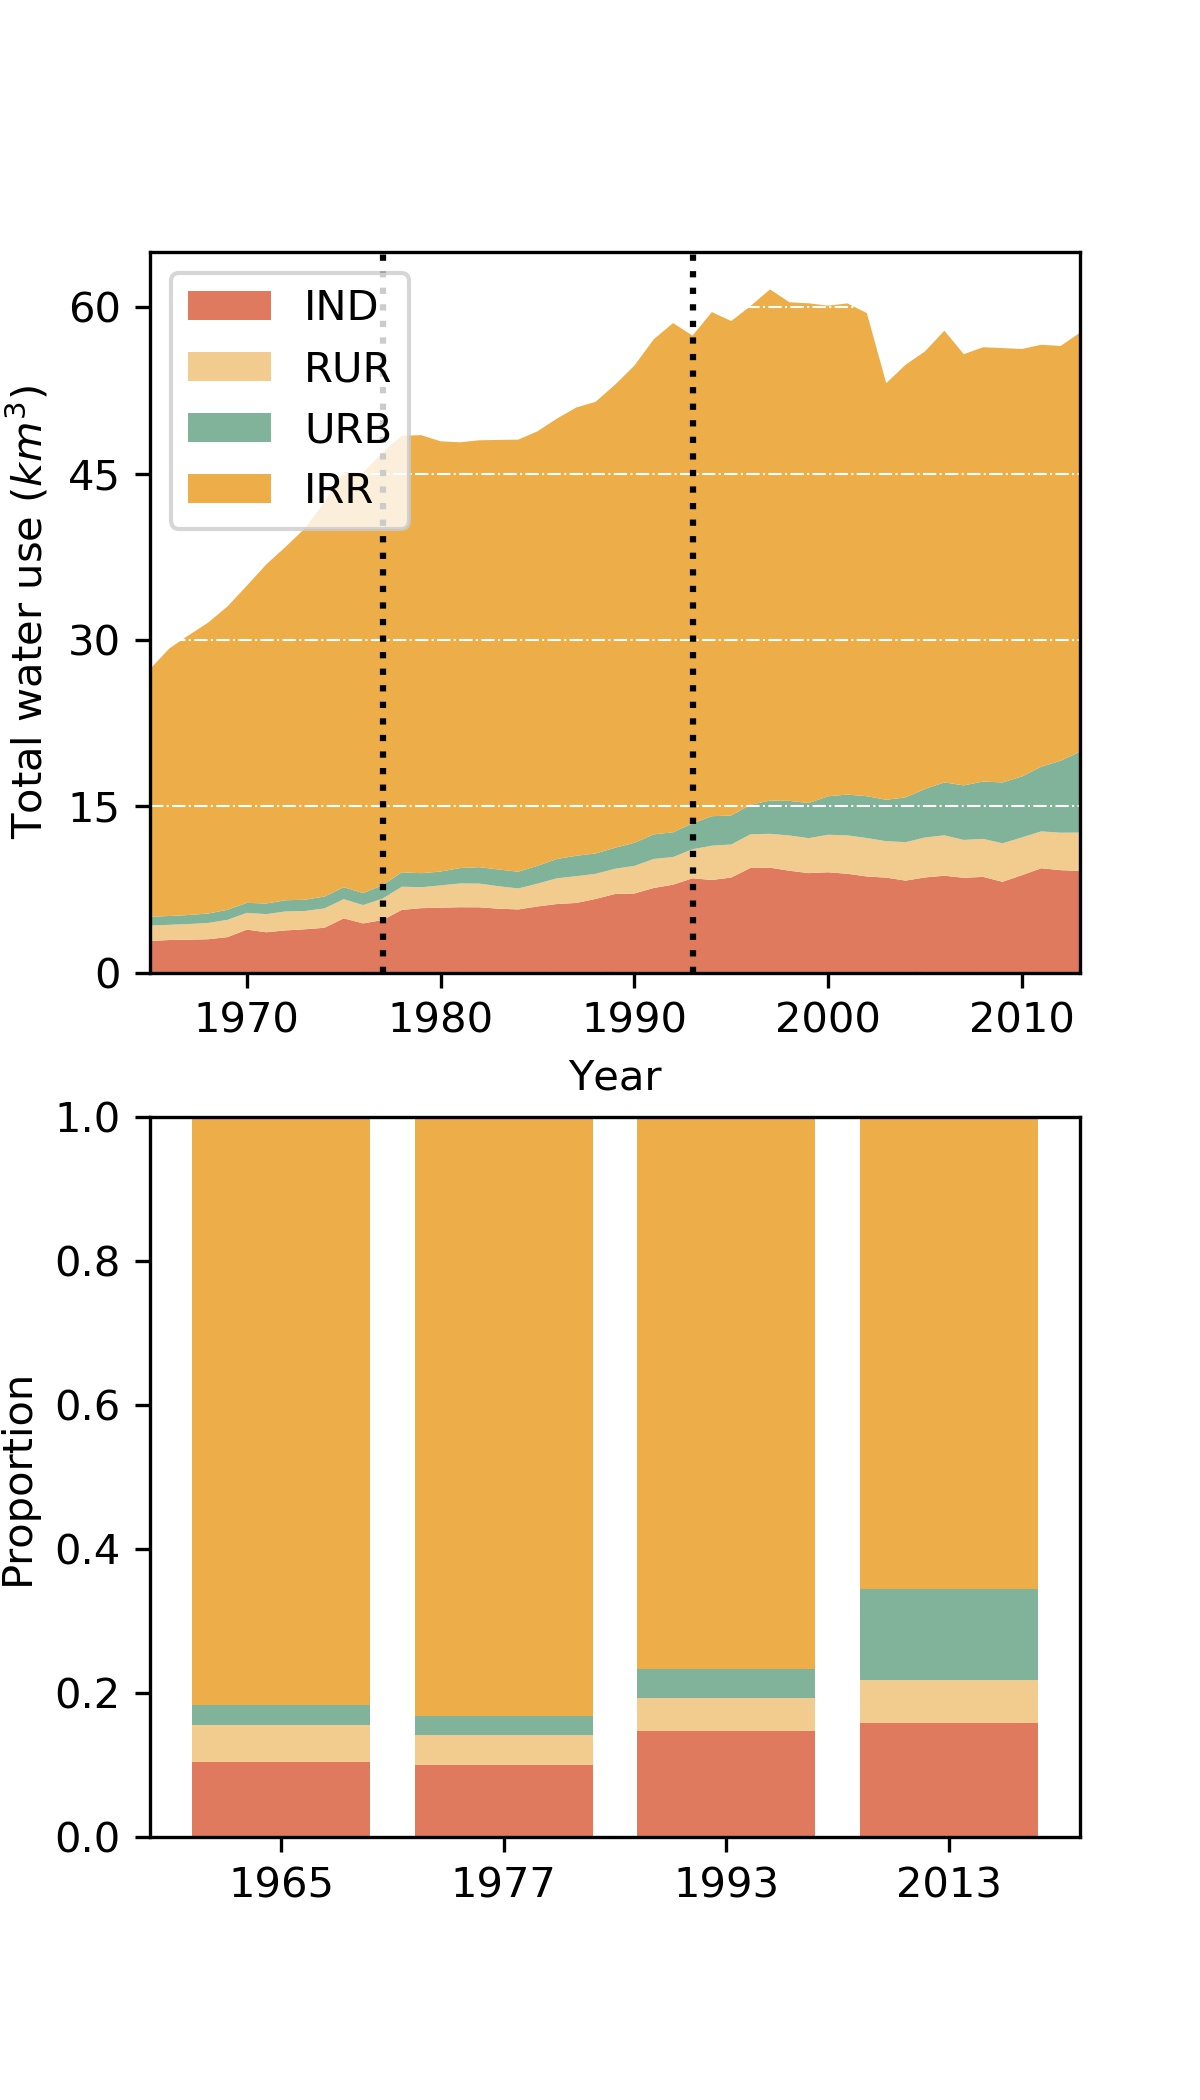
\includegraphics[width=0.6\textwidth]{../../figures/supplementary_information/sf_wu_sections_stackplot.jpg}
    \caption{Proportions of water use between the different sectors}
\end{figure}

% 补充图片8:黄河断流
\begin{figure}
    \centering
    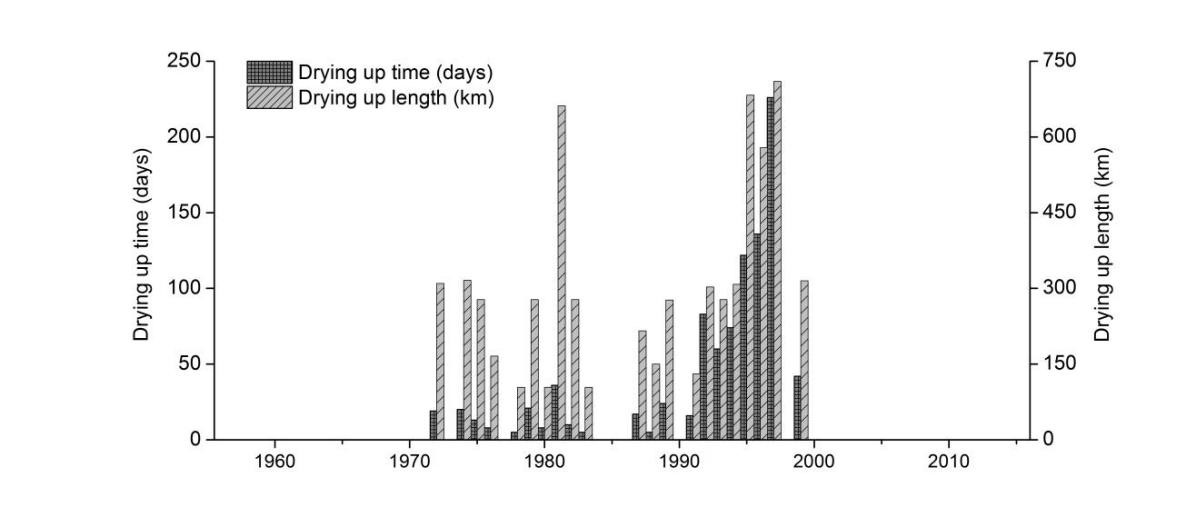
\includegraphics[width=0.95\textwidth]{../../figures/supplementary_information/outages.jpg}
    \caption{Severe runoff outages and groundwater depletion}
\end{figure}

% 补充图片9:管理政策
\begin{figure}
    \centering
    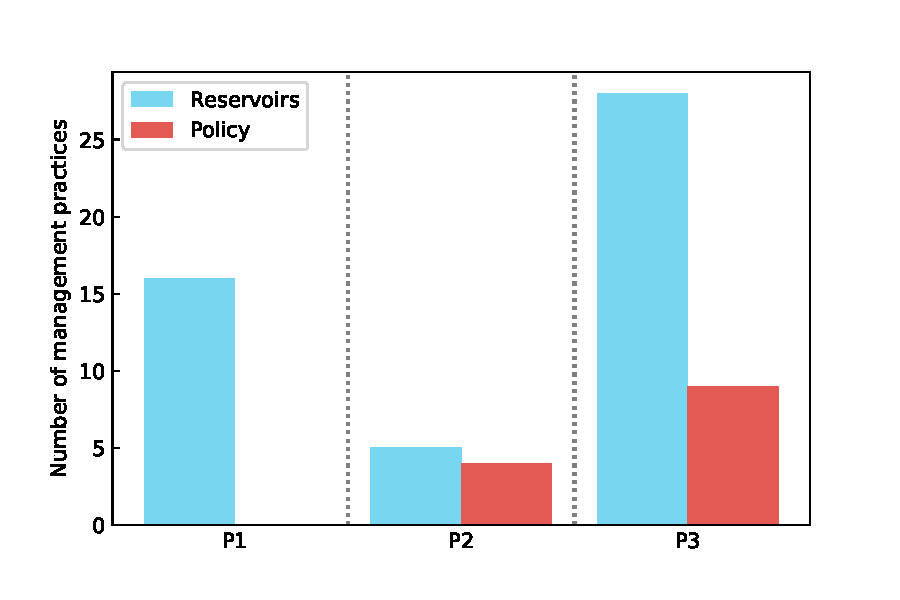
\includegraphics[width=0.95\textwidth]{../../figures/supplementary_information/managements.pdf}
    \caption{Number of management practices in different periods, including policy and reservoirs.}
\end{figure}



% %% 表格
% \begin{table}\centering
% \caption{This is a table}

% % 表格
% \begin{tabular}{lrrrr}
% Species & CBS & CV & G3 \\
% \midrule
% 1. Acetaldehyde & 0.0 & 0.0 & 0.0 \\
% 2. Vinyl alcohol & 9.1 & 9.6 & 13.5 \\
% 3. Hydroxyethylidene & 50.8 & 51.2 & 54.0\\
% \bottomrule
% \end{tabular}
% \end{table}



%% 表格
\begin{table}\centering
    \caption{Used datasets and their sources.}
    
    % 表格
    \begin{tabular}{lrrrr}
    Dataset & Type & Spatial scale & Time limit & Source \\
    \midrule
    1. Water use & Statistical & Perfects & 1965-2013 & 2nd National Water Resources Assessment Program \\
    2. GDP & Statistical & Province & 1949-2019 & Wind database \\
    3. Groundwater and surface water use & Statistical & Watershed & 2003-2019 & Yearbooks of YRB by the YRCC. \\
    \bottomrule
    \end{tabular}
\end{table}



%%% Add this line AFTER all your figures and tables
\FloatBarrier

% \dataset{dataset_one.txt}{Type or paste legend here.}

% \dataset{dataset_two.txt}{Type or paste legend here. Adding longer text to show what happens, to decide on alignment and/or indentations for multi-line or paragraph captions.}

\bibliography{pnas-sample}

\end{document}